%!TEX program = xelatex
% Please make sure you insert your
% data according to the instructions in PoSauthmanual.pdf
\documentclass[a4paper,11pt]{article}
\usepackage{pos}
\usepackage{wrapfig}
\usepackage{bbm}
\usepackage{natbib}
\usepackage{amsfonts}
\usepackage{amsmath}
\usepackage{graphicx}% Include figure files
\usepackage{dcolumn}% Align table columns on decimal point
\usepackage{bm}% bold math
\usepackage[ruled, vlined]{algorithm2e}
\usepackage{silence}
\usepackage{subcaption}
\usepackage[normalem]{ulem}
% \reversemarginpar

\definecolor{blue}{HTML}{007fff}
\definecolor{red}{HTML}{FF2052}

\newcommand{\mask}{\textcolor{blue}{{m}}}
\newcommand{\maskbar}{\textcolor{red}{\bar{m}}}

\newcommand{\xm}{\textcolor{blue}{{x}}}
\newcommand{\xmbar}{\textcolor{red}{\bar{x}}}

\newcommand{\xmask}{\textcolor{blue}{{x}_{m}}}
\newcommand{\xmaskbar}{\textcolor{red}{x_{\bar{m}}}}

\newcommand{\xpmask}{\textcolor{blue}{{x'}_{m}}}
\newcommand{\xpmaskbar}{\textcolor{red}{x'_{\bar{m}}}}

\newcommand{\mbart}{\textcolor{red}{\bar{m}^{k}}}
\newcommand{\mt}{\textcolor{blue}{m^{k}}}
\newcommand{\gradS}{\partial_{x} S(x)}
\newcommand{\acceptProb}{%
            A(\xi^{\ast}|\xi) \equiv \min\left\{1,
            \frac{p(\xi^{\ast})}{p(\xi)}%
        \left|\frac{\partial \xi^{\ast}}{\partial \xi^{T}}\right|\right\}
    }

\newcommand{\mpar}[1]{\marginpar{\color{red}{#1}}}

\title{LeapfrogLayers: A Trainable Framework for Effective Topological Sampling}
% \ShortTitle{A Trainable Framework for effective Topological Sampling}

\author*[a]{Sam Foreman}
\author[a]{Xiao-Yong Jin}
\author[a]{James C. Osborn}

\affiliation[a]{Argonne National Laboratory,\\
  Lemont, IL}

% \affiliation[b]{Department, University,\\
% Street number, City, Country}

\emailAdd{foremans@anl.gov}
\emailAdd{xjin@anl.gov}
\emailAdd{osborn@alcf.anl.gov}

\abstract{
    We introduce LeapfrogLayers, an invertible neural network architecture that
    can be trained to efficiently sample the topology of a 2D $U(1)$ lattice
    gauge theory. 
    %
    We show an improvement in the integrated autocorrelation time of the
    topological charge when compared with traditional HMC, and propose methods
    for scaling our model to larger lattice volumes.
}

\FullConference{
  The 38th International Symposium on Lattice Field Theory\\
  26-30 July 2021\\
  Zoom / Gather @ MIT, Cambridge MA, USA\\
}

%% \tableofcontents
\begin{document}
\maketitle


\section{\label{sec:intro}Introduction}
%
\marginpar{\textcolor{red}{Background}}
%
One of the major goals of lattice field theory calculations is to evaluate
integrals of the form
%
\begin{equation}
    \langle \mathcal{O} \rangle \propto \int \left[ \mathcal{D} x \right] \mathcal{O}(x) p(x),
    \label{eq:density_integral}
\end{equation}
%
for some target distribution \(p(x)\propto e^{-S(x)}\).
%
We can approximate the integral using Markov Chain Monte Carlo (MCMC) sampling
techniques.
%
This is done by sequentially generating a chain of configurations \(\{x_{1},
x_{2}, \ldots x_{N}\}\), with \(x_{i} \sim p(x)\) and averaging the value of
the function \(\mathcal{O}(x)\) over the chain.
%
Accounting for correlations between states in our chain, the sampling variance
of this esimator is given by
%
\begin{equation}
    \sigmaup^{2} = \frac{\tau_{\mathcal{O}}^{\mathrm{int}}}{N}\sum_{n=1}^{N} \mathrm{Var}\left[\mathcal{O}(x)\right]
\end{equation}
%
% TODO: Elaborate on this
where \(\tau_{\mathrm{int}}^{\mathcal{O}}\) is the integrated autocorrelation
time.
%
This quantity can be interpreted as the additional time required for
these induced correlations to become negligible.
%
\subsection{\label{subsec:qfreezing}Charge Freezing}
%
\begin{wrapfigure}[23]{r}[40pt]{0.52\textwidth}
    \vspace{-\baselineskip}
    \centering
    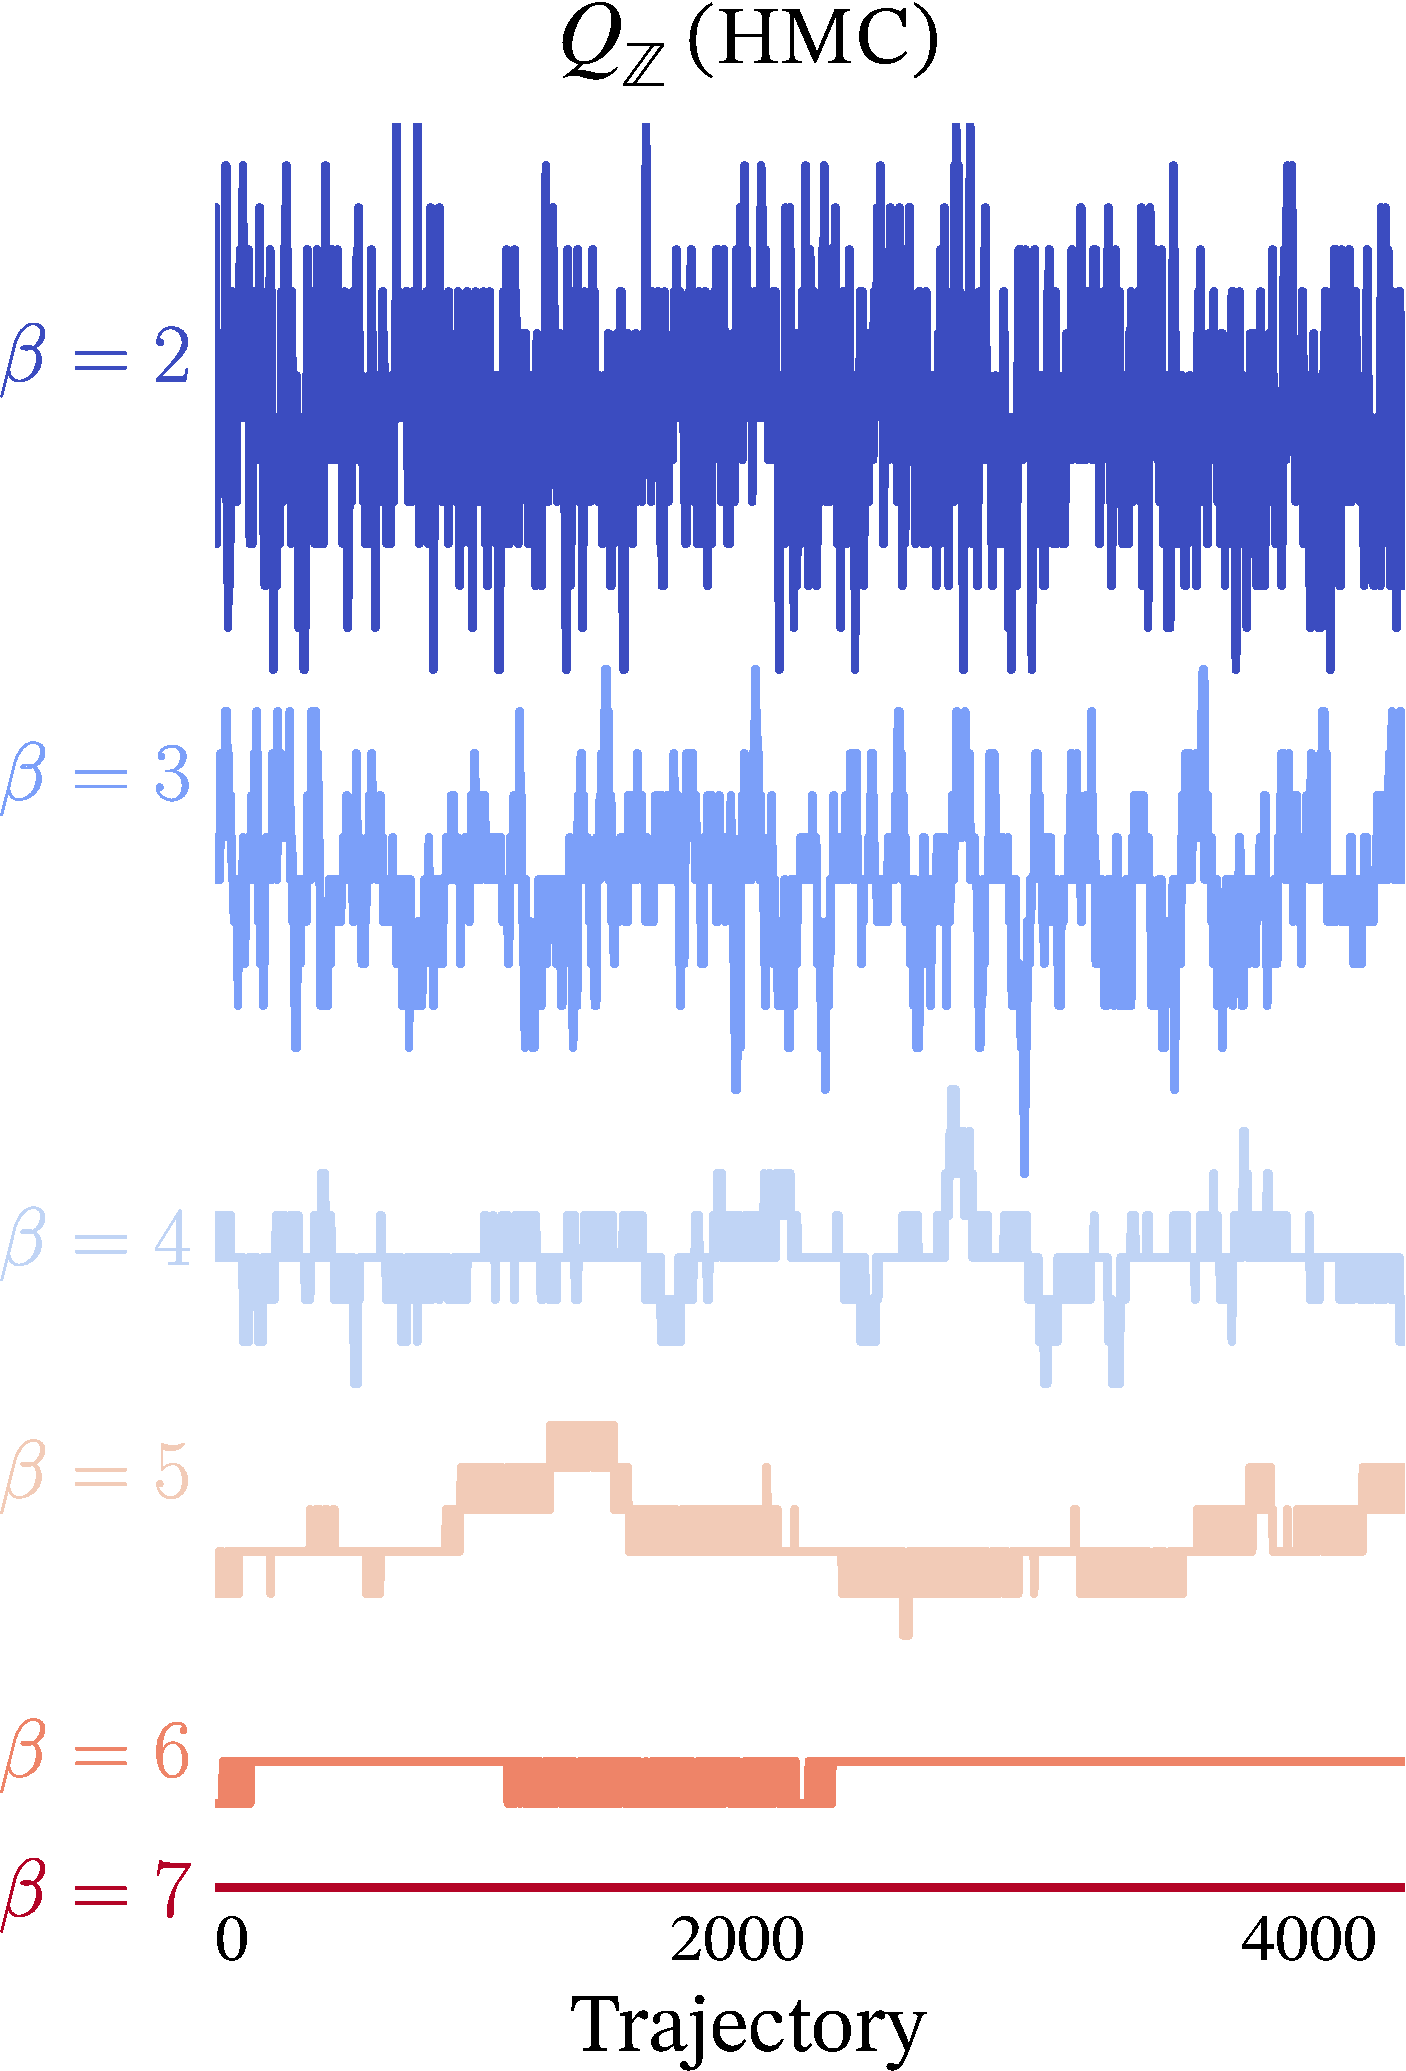
\includegraphics[width=0.52\textwidth]{assets/qfreezing.pdf}
    \caption{\label{fig:qfreezing}Illustration of the topological charge \(Q\)
    freezing as \(\beta : 2 \rightarrow 7\) for traditional HMC.}
\end{wrapfigure}
%
The ability to efficiently generate independent configurations is currently
a major bottleneck for lattice simulations.
%
In this work we consider a \(U(1)\) gauge model on a 2D lattice with periodic
boundary conditions.
%
The theory is defined in terms of the link variables \(U_{\mu}(x) = e^{i
x_{\mu}(n)} \in U(1)\) with \(x_{\mu}(n) \in [-\pi, \pi]\).
%
Our target distribution is given by \(p(x)\propto e^{-S_{\beta}(x)}\), where
\(S_{\beta}(x)\) is the Wilson action
%
\begin{align}
    S_{\beta}(x) &= \beta \sum_{P} 1 - \cos{x_{P}}, \text{    and}\\
    x_{P} &\equiv \big[x_{\mu}(n) + x_{\nu}(n + \hat{\mu})\nonumber
          % \quad\quad\,\, 
      - x_{\mu}(n+\hat{\nu}) - x_{\nu}(n)\big],
\end{align}
%
is the sum of the gauge variables around the elementary plaquette.
%
For a given lattice configuration, we can calculate the topological charge \(Q
\in \mathbb{Z}\) using
%
\begin{align*}
    Q_{\mathbb{Z}} &= \frac{1}{2\pi}\sum_{P}\left\lfloor x_{P} \right\rfloor,\text{ where } \\
    \left\lfloor x_{P} \right\rfloor &\equiv x_{P} - 2\pi
    \left\lfloor\frac{x_{P}+\pi}{2\pi}\right\rfloor.
\end{align*}
%
As \(\beta \rightarrow \infty\), the \(Q_{\mathbb{Z}} = 0\) mode becomes
dominant and we see that the value of \(Q_\mathbb{Z}\) remains fixed for large
durations of the simulation.
%

This can be seen by introducing the \emph{tunneling rate}\footnote{As measured
between subsequent states in our chain \(i\), \(i+1\).}
%
\begin{equation}
    \delta Q \equiv \left|Q_{i+1} - Q_{i}\right| \in \mathbb{Z},
\end{equation}
%
which serves as a measure for how efficiently our chain is able to jump
(tunnel) between sectors of distinct topological charge.
%
From Fig~\ref{fig:qfreezing}, we can see that \(\delta Q\rightarrow 0\) as
\(\beta\rightarrow \infty\).
%
\section{\label{sec:hmc}Hamiltonian Monte Carlo (HMC)}
%
The Hamiltonian Monte Carlo algorithm begins by introducing a fictitious
momentum \(v \sim \mathcal{N} (0, \mathbbm{1})\) distributed independently of
\(x\).
%
This allows us to write the joint target density of the \(\xi \equiv (x, v)\)
system as
%
\begin{equation}
    p(x, v) = p(x) \cdot p(v) = e^{-S_{\beta}(x)}\cdot e^{-v^{T} v / 2} = e^{-\mathcal{H} (x, v)}
\end{equation}
%
where \(\mathcal{H}(\xi) = \mathcal{H}(x, v) = S_{\beta}(x) + \frac{1}{2} v^{T}
v\) is the Hamiltonian of the system.
%
We use the \emph{leapfrog integrator} to numerically integrate Hamilton's
equations
%
\begin{equation}
    \dot{x} = \frac{\partial \mathcal{H}}{\partial v}\quad \text{,} \quad
    \dot{v} = - \frac{\partial \mathcal{H}}{\partial x}
\end{equation}
%
along iso-probability contours of \(\mathcal{H} =\text{const.}\) from \(\xi = (x,
v)\rightarrow (x^{\ast}, v^{\ast}) = \xi^{\ast}\).
%
\subsection{\label{subsec:lfint}Leapfrog Integrator}
%
\begin{enumerate}
    \item Starting from \(x_{0}\), resample the momentum \(v_{0}\sim
        \mathcal{N} (0, \mathbbm{1})\) and construct the state \(\xi =
        (x, v)\).
    \item Generate a \emph{proposal configuration} \(\xi^{\ast}\) by
        integrating \(\dot\xi\) along \(\mathcal{H} = \mathrm{const.}\)
        for \(N\) leapfrog steps.
        i.e.
        \begin{equation}
            \xi \rightarrow \xi_{1}\rightarrow\ldots\rightarrow
            \xi_{N} \equiv \xi^{\ast},
        \end{equation}
        where a single leapfrog step \(\xi_{i} \rightarrow \xi_{i+1}\) above
        consists of: 
        %
        \begin{equation}
            \textbf{ (a.) }%
              \tilde{v}\leftarrow v - \frac{\varepsilon}{2}\partial_{x} S(x),
            \quad\quad
            \textbf{ (b.) }%
              x' \leftarrow x + \varepsilon \tilde{v},
            \quad\quad
            \textbf{ (c.) }%
              v' \leftarrow \tilde{v} - \frac{\varepsilon}{2}\partial_{x} S(x).
        \end{equation}
        %
    \item At the end of the trajectory, accept or reject the proposal
        configuration \(\xi^{\ast}\) using the Metropolis-Hastings (MH) test
        \begin{equation}
            x_{i+1} \leftarrow
            \begin{cases}
                x^{\ast}\text{ with probability } \acceptProb \\
                x_{i}\text{ with probability } 1 - A(\xi^{\ast}|\xi).
            \end{cases}
        \end{equation}
\end{enumerate}
%
An illustration of this procedure can be seen in Fig~\ref{fig:hmc}.
%
\begin{figure}[htpb]
    \centering
    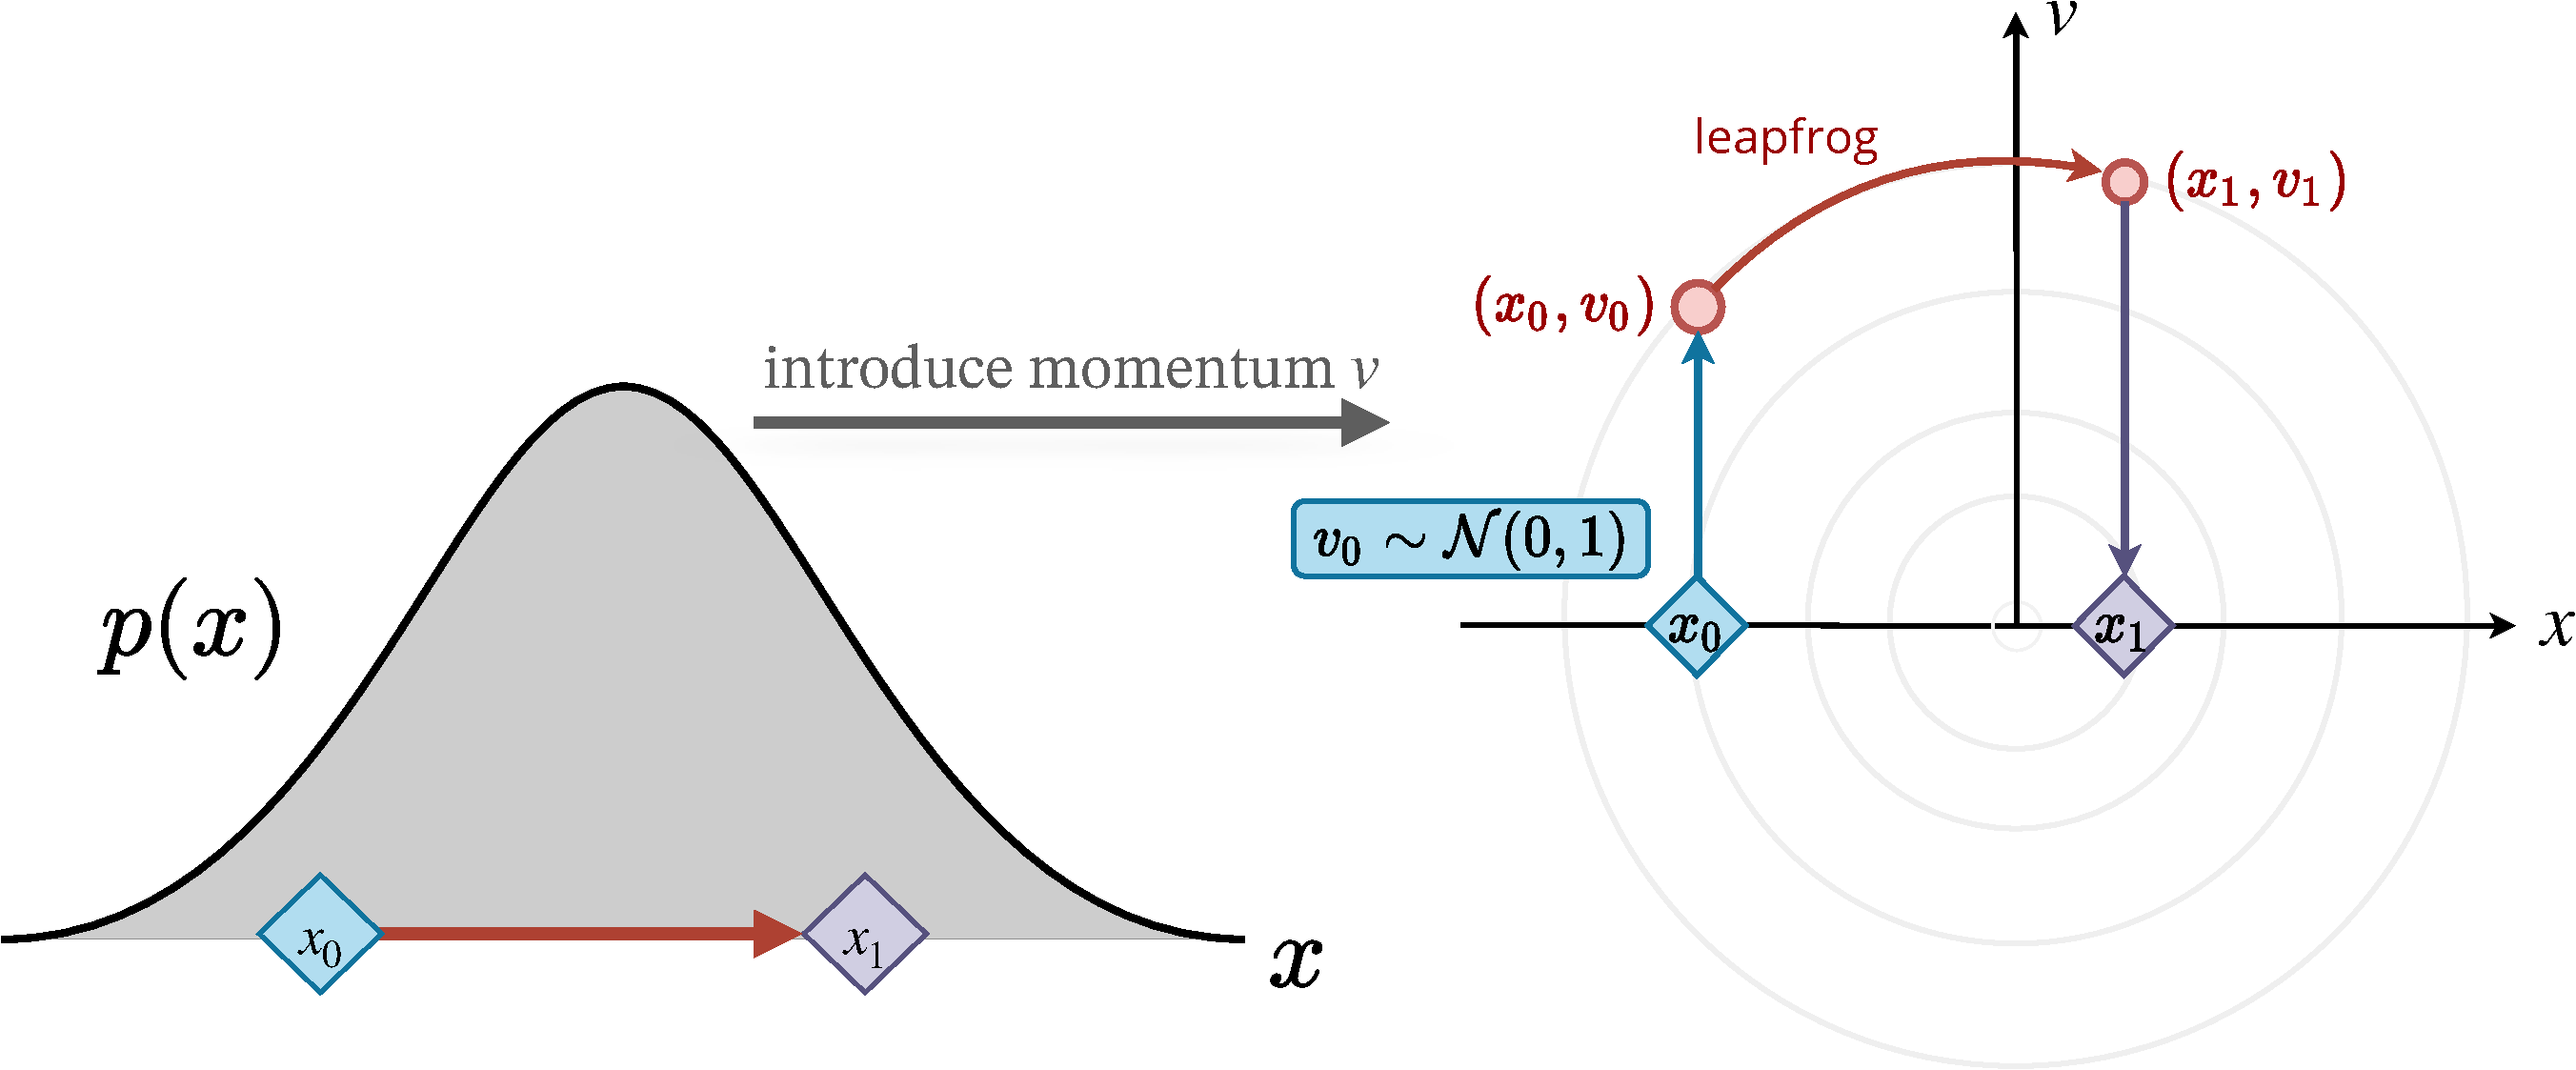
\includegraphics[width=\textwidth]{assets/hmc.pdf}
    \caption{\label{fig:hmc}High-level overview of the HMC algorithm.}
\end{figure}
%
\subsection{\label{subsec:hmc_issues}Issues with HMC}
%
Re-sampling the momentum at the start of each trajectory causes the energy
levels we explore to be randomly selected.
%
This is reminiscient of the ``random-walk'' behavior of traditional MCMC and
leads to a slow exploration of our target distribution (i.e. long
autocorrelations).
%
Additionally, the HMC sampler is known to have difficulty traversing
low-density zones, resulting in poor performance for distributions which have
multiple isolated modes.
%
This is particularly relevant in the case of sampling topological quantities in
lattice gauge models.
%
%
% This list of criteria helps to illuminate the qualities we would like our
% (ideal) sampler to exhibit; namely, we would like for our sampler to: 
% %
% \begin{itemize}
%     \item quickly converge to the true target distribution
%     \item mix quickly once converged (short autocorrelations)
%     \item be able to mix across energy levels and isolated modes
% \end{itemize}
%
\section{\label{sec:l2hmc}Generalizing HMC: LeapfrogLayers}
%
In order to preserve the asymptotic behavior of HMC, our update must be
explicitly reversible with a tractable Jacobian determinant.
%
% \begin{enumerate}
%     \item Be invertible / preserve reversibility, i.e. \(p(a\rightarrow b) =
%         p(b\rightarrow a)\)
%     \item Have a tractable Jacobian determinant.
% \end{enumerate}
% %
To simplify notation, we introduce two functions, \(\Gamma\) \((\Lambda)\) to
denote the \(v\) \((x)\) updates.
%
As in HMC, we follow the general pattern of performing alternating updates of
\(v\) and \(x\).
%

We can ensure our update is reversible by splitting the \(x\)-update into two
parts and sequentially updating complementary subsets using a binary mask
\(\mask\) and its complement \(\maskbar\).
%
As in~\cite{2017arXiv171109268L,Foreman:2021ixr}, we introduce \(d \sim
\mathcal{U} (+, -)\), distributed independently of both \(x\) and \(v\), to
determine the ``direction'' of our update\footnote{%
  As indicated by the superscript \(\pm\) on \(\Gamma^{\pm}, \Lambda^{\pm}\) in
  the update functions.
}.
%
Here, we associate \(+\) \((-)\) with the forward (backward) direction and note
that running sequential updates in opposite directions has the effect of
inverting the update.
%
We denote the complete state by \(\xi = (x, v, \pm)\), with target density
given by \(p(\xi) = p(x)\cdot p(v)\cdot p(\pm)\).
%

Explicitly, we can write this series of updates as\footnote{%
  Here we denote by \(\xmask = \mask \odot x\) and 
  \(\xmaskbar = \maskbar \odot x\) with \(\mathbbm{1} = \mask + \maskbar\).
}
%
\begin{align}
    \nonumber
    \textbf{(a.)}\,\,\,\, v' 
        \gets \Gamma^{\pm}\left[v;\, \zeta_{v} \right]\hspace{75pt}
    \textbf{(b.)}\,\,\,\, x' 
        &\gets \mask \odot x + \maskbar \odot \Lambda^{\pm} [\xmaskbar; \zeta_{\bar{x}}] \\
    \nonumber
    \textbf{(c.)}\,\, x'' 
        \gets \maskbar \odot x' + \mask \odot \Lambda^{\pm} [\xmask; \zeta_{x'}] \quad
    \textbf{(d.)}\,\, v'' 
        &\gets \Gamma^{\pm} [v', \zeta_{v'}]
\end{align}
%
where \(\zeta_{\bar{x}} = [\maskbar\odot x, v]\), \(\zeta_{x} = [\mask \odot x,
v]\) \((\zeta_{v} = [x, \partial_{x} S(x)])\) is independent of \(x\) \((v)\)
and is passed as input to the update functions \(\Lambda^{\pm}\)
\((\Gamma^{\pm})\).
%
\begin{figure}[htpb]
    \centering
    \begin{subfigure}[b]{0.40\textwidth}
        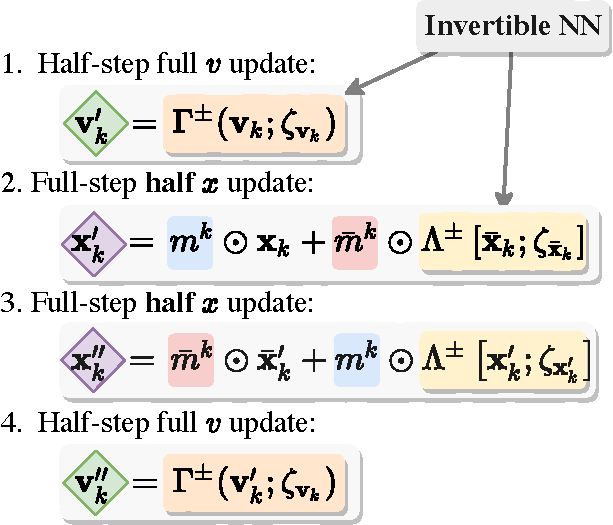
\includegraphics[width=\textwidth]{assets/update_steps.pdf}
        \caption{\label{subfig:updates}Generalized leapfrog update.}
    \end{subfigure}
    \hfill
    \begin{subfigure}[b]{0.55\textwidth}
        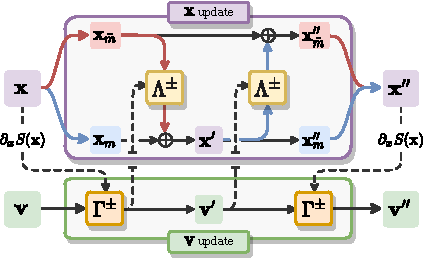
\includegraphics[width=\textwidth]{assets/leapfrog_layer.pdf}
        \caption{\label{subfig:lfupdate}Illustration of the data flow
        through a leapfrog layer.}
    \end{subfigure}
    % \vspace{1em}
    \begin{subfigure}[t]{\textwidth}
        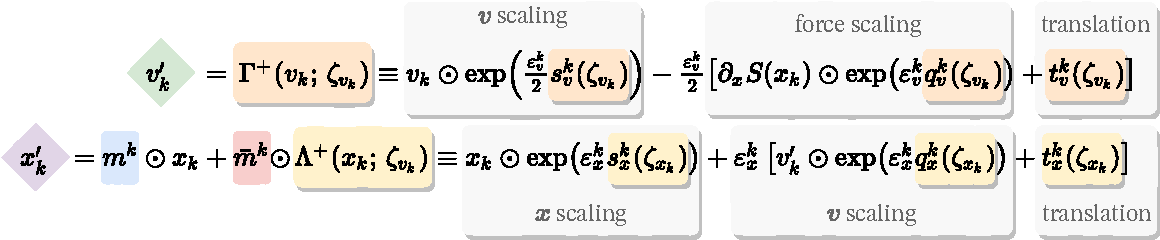
\includegraphics[width=0.98\textwidth]{assets/network_functions.pdf}
        \caption{\label{subfig:network_fns}Detailed view of the first two steps
        in Fig~\ref{subfig:updates}. Note that \(k\) indexes the leapfrog step
    along our trajectory.}
    \end{subfigure}
    \caption{\label{fig:networks}Various illustrations of the generalized
    leapfrog update.}
\end{figure}
%
%     of the leapfrog layer used
%     to generate a proposal configuration \(\xi\rightarrow \xi''\) which is
% then either accepted or rejected.}
%     which uses invertible neural networks to augment the
% traditional update.}
%
\subsection{\label{subsec:networks}Network Details}
%
Normalizing flows~\cite{DinhSB16} are an obvious choice
for the structure of the update functions.
%
These architectures are easily invertible while maintaining a tractable
Jacobian determinant, and have also been shown to be effective at approximating
complicated target distributions in high-dimensional spaces ~\cite{%
    Foreman:2021ixr,%
    Kanwar:2020xzo,%
    DinhSB16,%
    Albergo:2021vyo,%
    Boyda:2020hsi,%
    2017arXiv171109268L,%
    2020arXiv201008047N,%
    2020arXiv200616653N,%
    2020arXiv200600866W%
    % neklyudovOrbitalMCMC2020a,%
    % wehenkelYouSayNormalizing2020a,%
    % neklyudovInvolutiveMcmcUnifying2020a%
}.

Note that we maintain separate networks \(\Gamma\), \(\Lambda\) with
identical architectures for updating \(v\) and \(x\), respectively.
%
Without loss of generality, we describe below the details of the \(x\)-update
for the forward \((d = +)\) direction, \(\Lambda^{+}[\xmaskbar;
\zeta_{\bar{x}}]\)\footnote{
    To get the update for the \(d=-\) direction, we invert the
    update functions and run them in the opposite order.
}.
%
For simplicity, we describe the data flow through a single leapfrog layer,
%
which takes as input \(\zeta_{\bar{x}} = (\xmaskbar, v)\).
%
For the 2D \(U(1)\) model, the gauge links are encoded as \([\cos(x),
\sin(x)]\) for \(x \in [-\pi, \pi]\).
%
Explicitly\footnote{
    Here \(\sigma(\cdot)\) is a generic nonlinear activation function.
},
%
\begin{align}
    h_{1} &= \sigma\left(w_{x}^{T} x + w_{v}^{T} v + b_{1}\right)
        \quad \in \mathbb{R}^{n_{1}} \\
    h_{2} &= \sigma\left(w_{2}^{T} h_{1} + b_{2}\right)
        \hspace{0.085\textwidth} \in \mathbb{R}^{n_{2}} \\
    \nonumber \vdots & \\
    h_{k} &= \sigma\left(w_{k}^{T} h_{k-1} + b_{k-1}\right)
        \hspace{0.04\textwidth} \in \mathbb{R}^{n_{k}} \Longrightarrow \\
    \nonumber
    \textbf{  (a.)  } s_{x} = \lambda_{s} \tanh \left( w^{T}_{s} h_{k} + b_{s} \right);
    &\quad\textbf{  (b.)  } t_{x} = w^{T}_{t} h_{k} + b_{t};
    \quad\textbf{  (c.)  } q_{x} = \lambda_{q}\tanh\left(w^{T}_{q} h_{k} + b_{q}\right);
\end{align}
%
where the outputs \(s_{x}, t_{x}, q_{x}\) are of the same dimensionality as
\(x\), and \(\lambda_{s}, \lambda_{q}\) are trainable parameters.
%
% Note that the shapes of the hidden layers \(h_{k}\) are determined by the sizes
% of each of the weight matrices \(w_{k}^{T}\).
% %
These outputs are then used to update \(x\), as shown in
Fig~\ref{fig:networks}.

\subsection{\label{subsec:training}Training Details}
%
To train the network, our goal is to train a sampler that efficiently
jumps between different topological charge sectors.
%
This can be done by constructing a loss function that maximizes the expected
squared charge difference between the initial \((\xi)\) and proposal
\((\xi^{\ast})\) configuration generated by the sampler.
%
Explicitly, we define
%
\begin{equation}
    \mathcal{L}_{\theta}(\xi^{\ast}, \xi) 
    = A(\xi^{\ast}|\xi) \cdot (Q^{\ast}_{\mathbb{R}} - Q_{\mathbb{R}})^{2}
\end{equation}
%
where \(Q_{\mathbb{R}} = \frac{1}{2\pi}\sum_{P} \sin x_{P} \in \mathbb{R}\) is
a real-valued approximation of the usual (integer-valued) topological charge
\(Q_{\mathbb{Z}} \in \mathbb{Z}\).
%
This ensures that our loss function is continuous which helps to simplify the
training procedure.
%
For completeness, the details of an individual training step are summarized in
Sec~\ref{subsubsec:trainstep}.
%
\subsubsection{\label{subsubsec:trainstep}Training Step}
%
\begin{enumerate}
    \item Resample \(v \sim \mathcal{N} (0, \mathbbm{1})\),
        \(d \sim \mathcal{U} (+, -)\), and construct initial state
        \(\xi = (x, v, \pm)\)
    \item Generate the proposal configuration \(\xi^{\ast}\) by passing the
        initial state sequentially through \(N\) \emph{leapfrog
        layers }%\footnote{
            %We defer the details to Sec~\ref{sec:l2hmc}.
        %}
        generate a proposal configuration: \(\xi \rightarrow \xi_{1}
        \rightarrow \ldots \rightarrow \xi_{N} = \xi^{\ast}\)
    \item Compute the Metropolis-Hastings acceptance \(A(\xi^{\ast} | \xi) =
        \min\left\{1, \frac{p(\xi^{\ast})}{p(\xi)}\left|\frac{\partial
        \xi'}{\partial \xi^{T}} \right| \right\}\)
    \item Evaluate the loss function \(\mathcal{L} \leftarrow
        \mathcal{L}_{\theta}(\xi^{\ast}, \xi)\), and backpropagate gradients to
        update weights
    \item Evaluate Metropolis-Hastings criteria and assign the next state in
        the chain according to
        \(x_{t+1} \leftarrow \begin{cases}%
            x^{\ast} \text{ with prob. } A(\xi^{\ast}|\xi) \\
            x \text{ with prob. } 1 - A(\xi^{\ast}|\xi).
        \end{cases}\)
\end{enumerate}
%
\subsubsection{\label{subsubsec:annealing}Annealing Schedule}
As an additional tool to help improve the quality of the trained sampler, we
introduce during the training phase an \emph{annealing schedule}:
\(\{\gamma_{t}\} = \{\gamma_{0}, \gamma_{1}, \ldots, \gamma_{N}\}\), where \(\gamma_{0} < \gamma_{1} < \cdots < \gamma_{N} \equiv 1\) and \(|\gamma_{i+1} - \gamma_{i}| \ll 1\).
%
For \(\|\gamma\| < 1\), this helps to rescale (shrink) the energy barriers
between isolated modes, and our target distribution becomes \(p_{t}(x) \propto
e^{-\gamma_{t} S(x)}\) for \(t = 0, 1, \ldots, N\).
%
\section{\label{sec:results}Results}
We can measure the performance of our approach by comparing the integrated
autocorrelation time against traditional HMC.
%
We see in Fig~\ref{fig:autocorr} that our estimate of the integrated
autocorrelation time is much shorter for the trained model across \(\beta \in
[2, 7]\).
%
\begin{figure}[htpb]
    \centering
    \begin{subfigure}[b]{0.47\textwidth}
        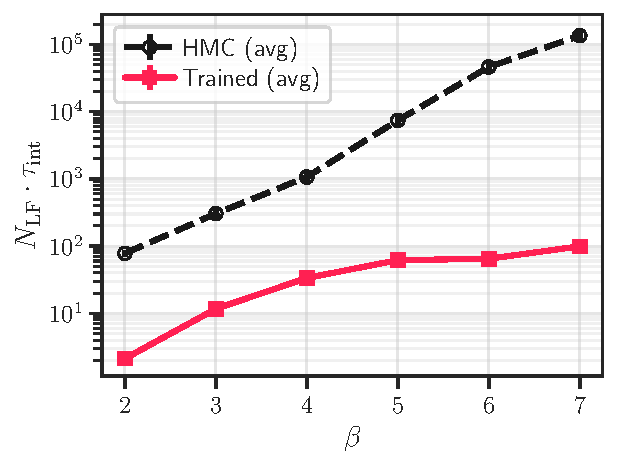
\includegraphics[width=\textwidth]{assets/autocorr_vs_beta.pdf}
        \caption{\label{fig:autocorr} The integrated autocorrelation
        time \(\tau_{\mathrm{int}}^{Q}\) vs \(\beta\)}
    %     of the topological charge for both HMC
    % (black, dashed line) and the trained model (solid, red line).}
    \end{subfigure}
    \hfill
    \begin{subfigure}[b]{0.49\textwidth}
        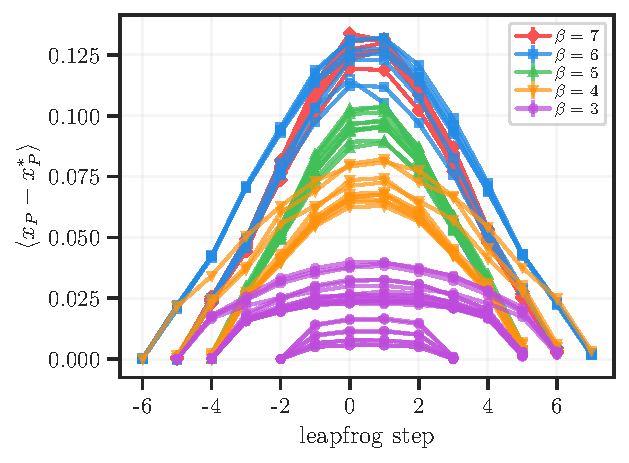
\includegraphics[width=\textwidth]{assets/plaqsf_leapfrog.pdf}
        \caption{\label{fig:plaqsf_beta}Deviation in the average plaquette vs
        leapfrog step.}
    \end{subfigure}
    \begin{subfigure}[b]{\textwidth}
        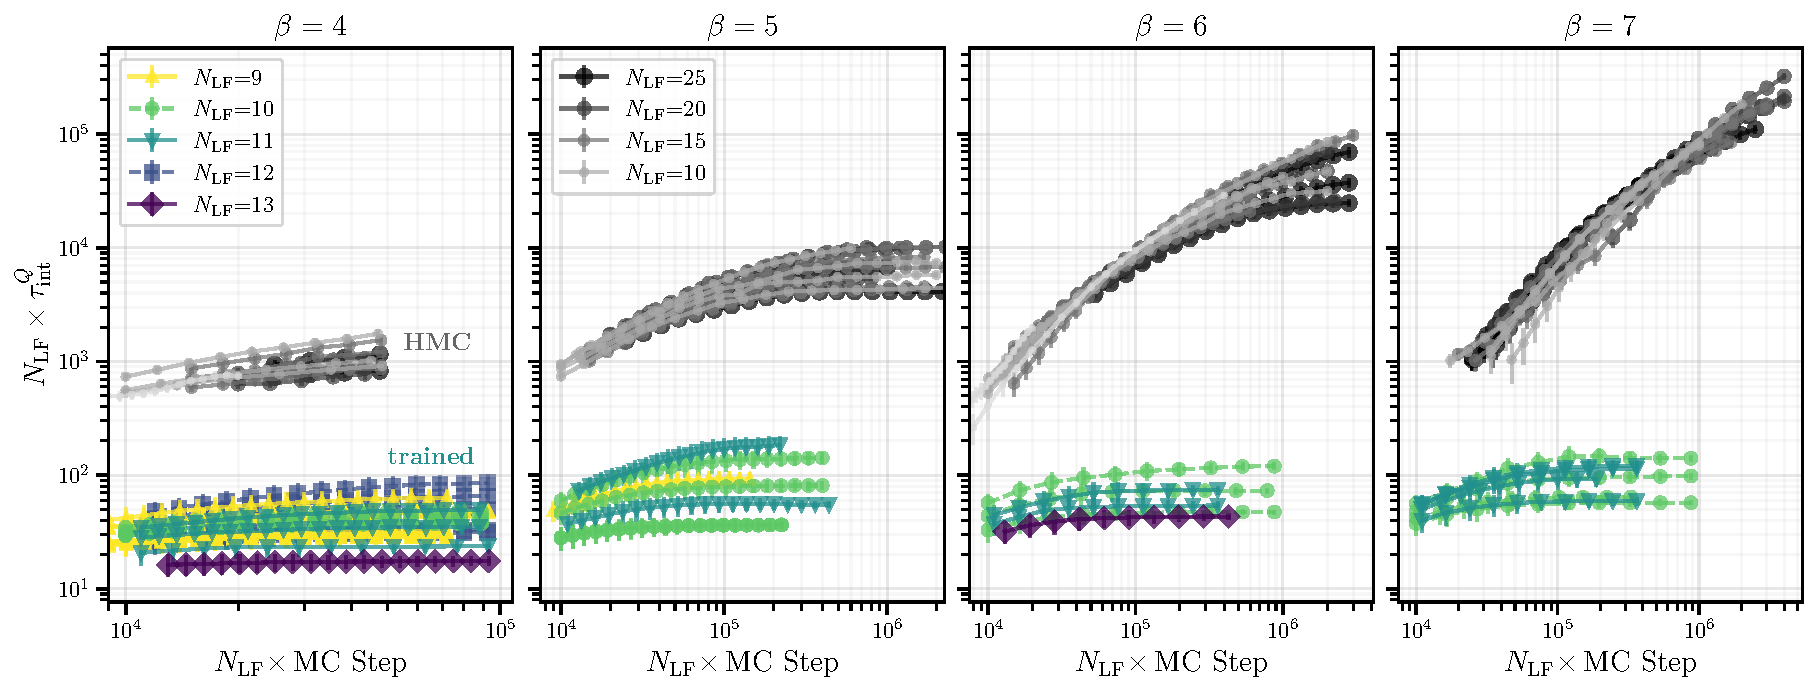
\includegraphics[width=\textwidth]{assets/tint.pdf}
        \caption{\label{fig:tint}Integrated autocorrelation time for trained
        models with different trajectory lengths \(N_{\mathrm{LF}}\), at
    \(\beta = 2, 3, \ldots, 7\)}
    \end{subfigure}
    \begin{subfigure}[t]{\textwidth}
        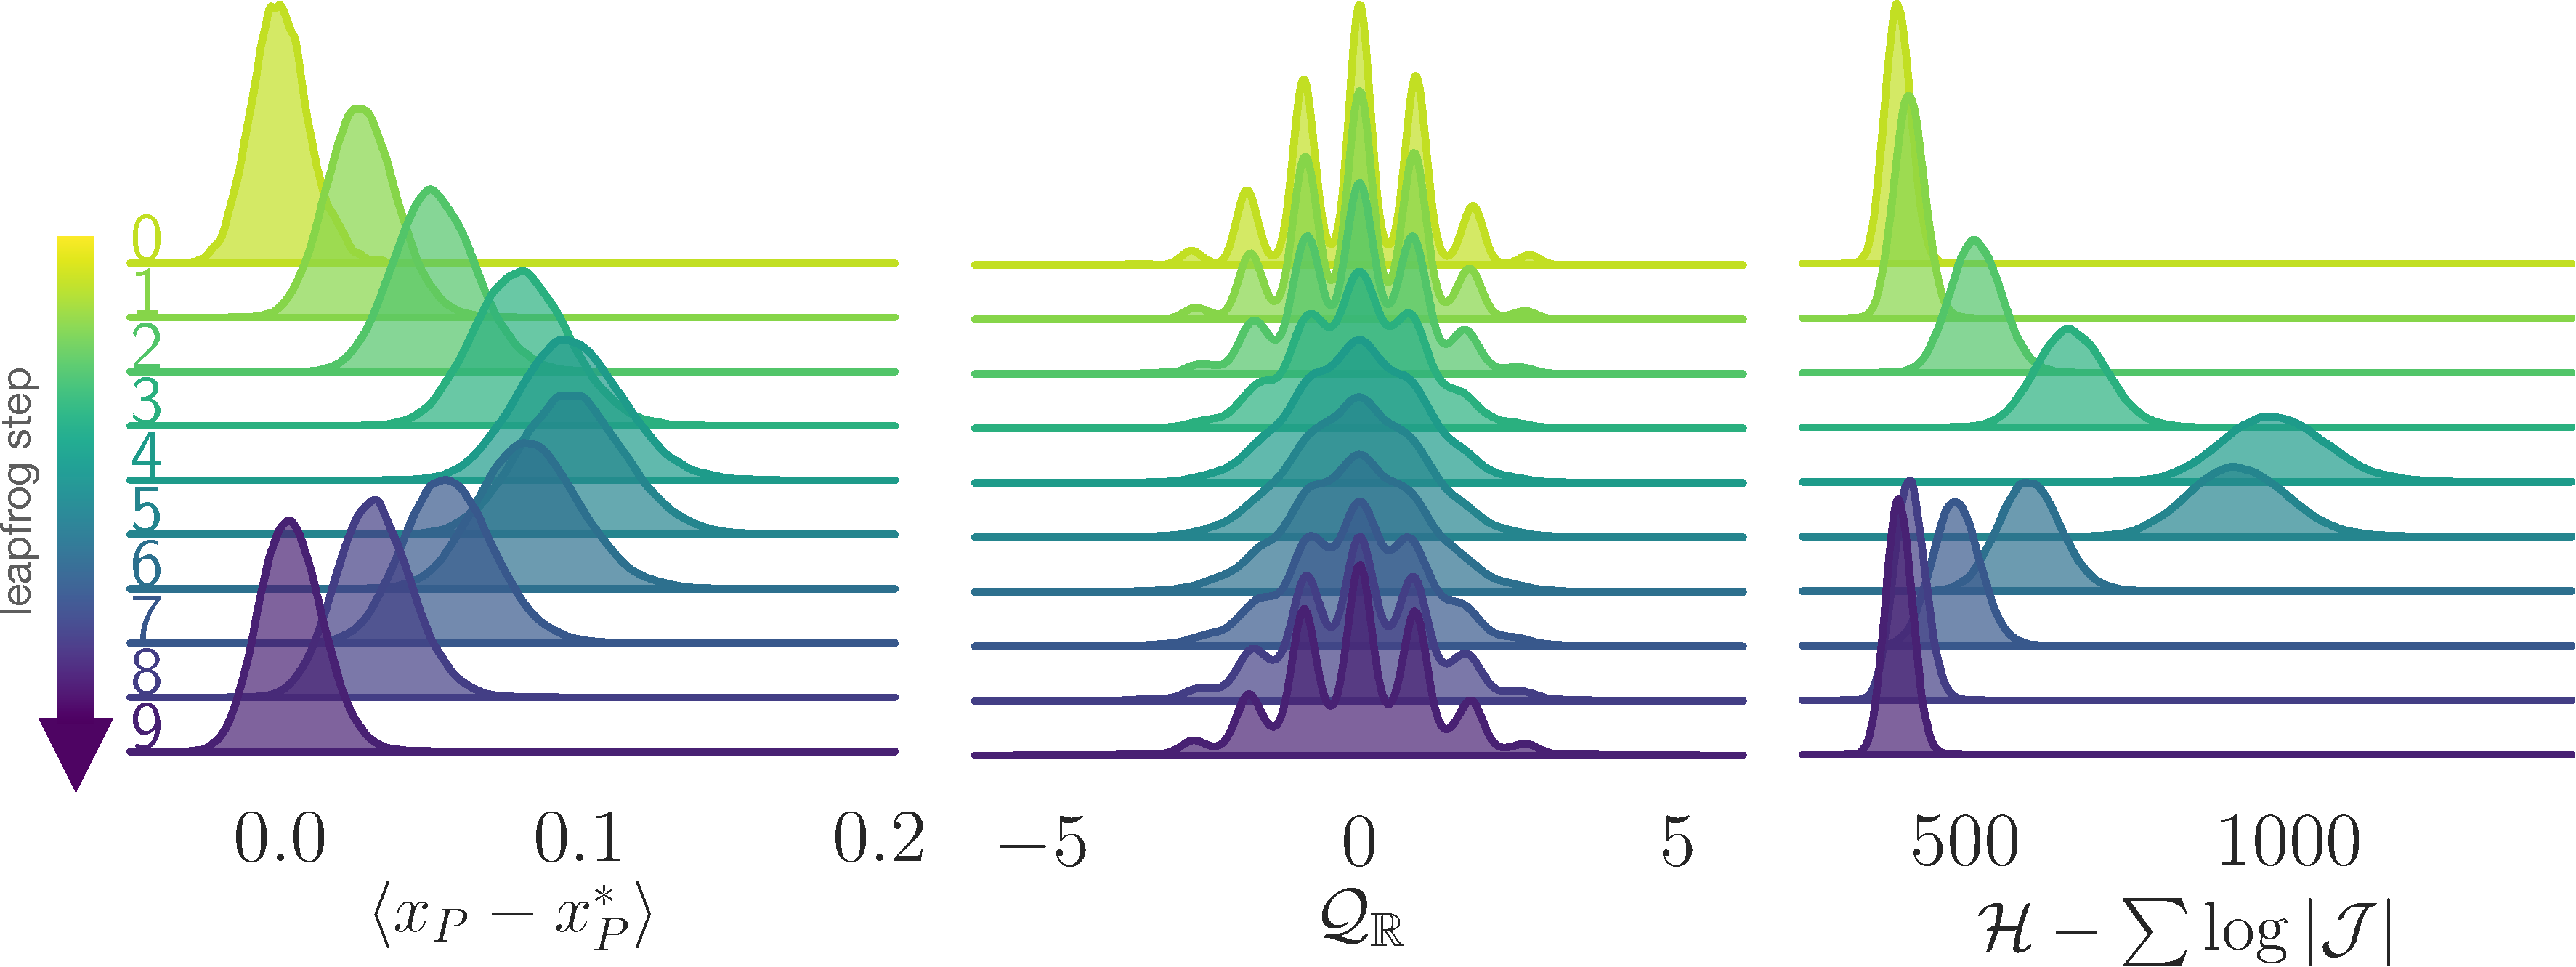
\includegraphics[width=\textwidth]{assets/ridgeplots.pdf}
        \caption{\label{fig:ridgeplots}Illustration of how different quantities
            change during the generalized leapfrog update, the variation in the
            average plaquette (left), the real-valued topological charge
        (middle) and the effective energy (right).}
    \end{subfigure}
    \caption{\label{fig:observables}Plots of various lattice observables.}
\end{figure}
%
% \begin{figure}[htpb]
%     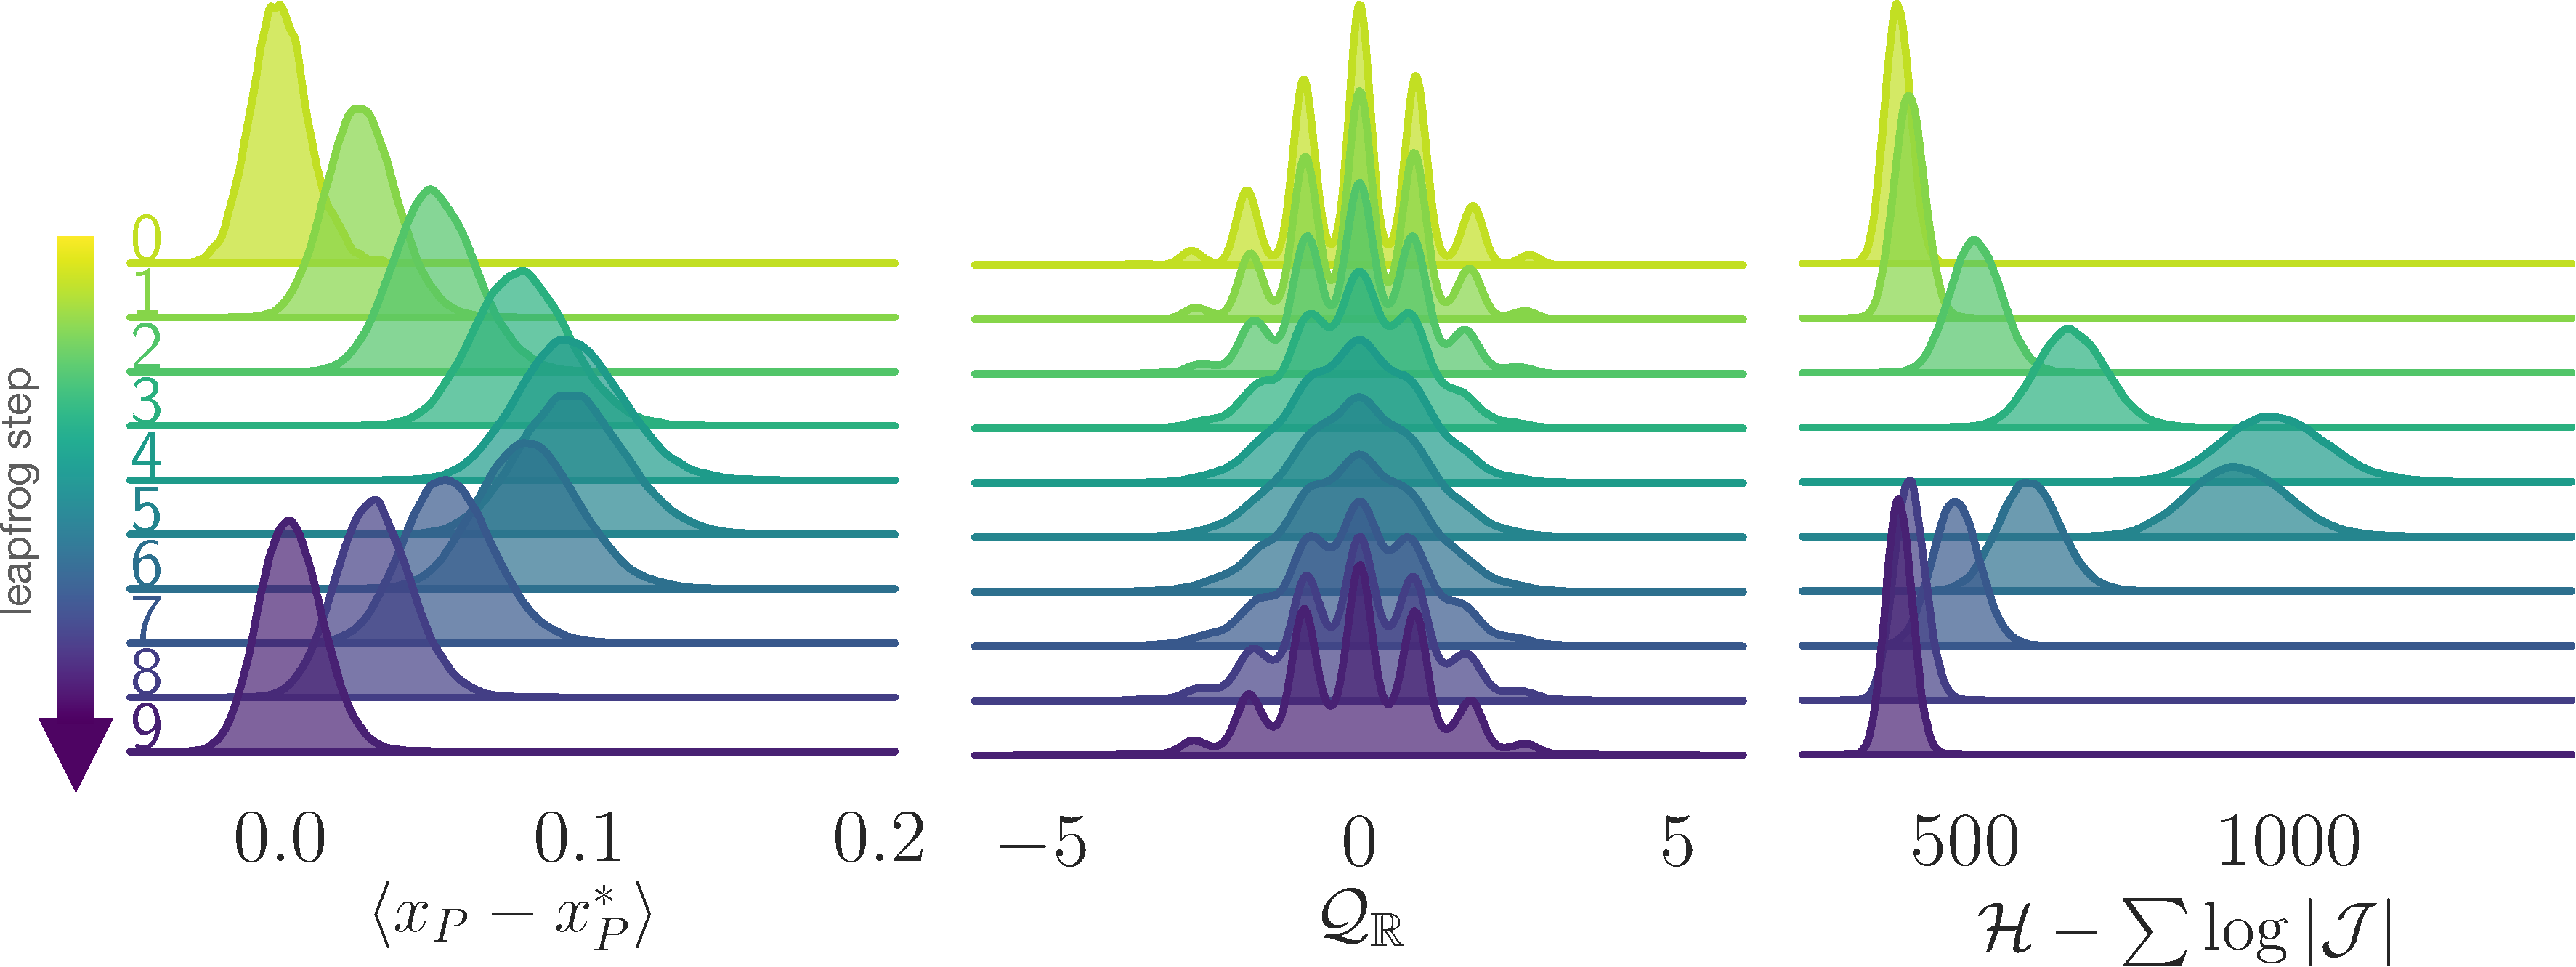
\includegraphics[width=\textwidth]{assets/ridgeplots.pdf}
%     \caption{\label{fig:ridgeplots}Illustration of how different quantities
%         change during the generalized leapfrog update, the variation in the
%         average plaquette (left), the real-valued topological charge
%     (middle) and the effective energy (right).}
% \end{figure}
%
To better understand how these transformations effect the HMC update, we can
look at how various quantities change over the course of a trajectory, as shown
in Fig~\ref{fig:ridgeplots}.
%

We see from the plot of \(\mathcal{H} - \sum \log | \mathcal{J} |\) in
Fig~\ref{fig:ridgeplots} (right) that the trained sampler artificially
increases the energy towards the middle of the trajectory.
%
This is analogous to reducing the coupling \(\beta\) during the trajectory, as
can be seen\footnote{%
    Note the trajectories have been shifted to be centered around their
    midpoints.
} in Fig~\ref{fig:plaqsf_beta}.
%
By looking at the variation in the average plaquette\footnote{%
    Here \(x^{\ast}_{P}\) denotes the expected value in the infinite volume limit.
} \(\langle x_{P} - x^{\ast}_{P}\rangle\) over a trajectory for models trained
at multiple values of beta we are able to better understand how our sampler
behaves.
%
This allows our trajectories to explore new regions of the target distribution
which may have been previously inaccessible.
%
\section{\label{sec:conclusion}Conclusion}
%
In this work we have proposed a generalized sampling procedure for HMC that can
be used for generating gauge configurations in the 2D \(U(1)\) lattice model.
%
We showed that our trained model is capable of outperforming traditional
sampling techniques across a range of inverse coupling constants, as measured
by the integrated autocorrelation time of the topological charge.
%
By looking at the evolution of different quantities over the generalized
leapfrog trajectory, we are able to gain insight into the mechanism driving
this improved behavior.
%

% Explicitly, if we denote by \(M^{\pm} = \left(\begin{smallmatrix}\Gamma^{\pm} &
% \cdot \\ \cdot & \Lambda^{\pm}\end{smallmatrix}\right)\), we have that 
% %
% \begin{equation}
%     \xi^{\pm} = M^{\pm}\xi \Longrightarrow \xi = M^{\mp}\xi^{\pm}.
% \end{equation}
% %

% \begin{thebibliography}{98}
\bibliography{main}
\bibliographystyle{plain}
% \bibitem{...}

% \end{thebibliography}

\end{document}
